\documentclass[../../main.tex]{subfiles}
\graphicspath{{\subfix{../images/}}} % 指定图片目录,后续可以直接使用图片文件名。
\begin{document}
\section{Homework 2}
\begin{enumerate}
  \item \textbf{Show that the volume element 
  \begin{align*}
    \mathrm{d}\omega = \prod_{i=1}^{3N}(\mathrm{d}q_{i}\mathrm{d}p_{i})
  \end{align*}
  of the phase space remains invariant under a canonical transformation of the (generalized) coordinates $(q,p)$ to any other set of (generalized) coordinates $(Q,P)$.}

  \textbf{[Hint: Before considering the most general transformation of this kind, which is referred to as a contact transformation, it may be helpful ti consider a point transformation - one in which the new coordinates $Q_{i}$ and the old coordinates $q_{i}$ transform only among themselves.]}
  \begin{align*}
    (Q,P) &= (Q(q,p),P(q,p))
  \end{align*}
  So the volume element is 
  \begin{align*}
    \mathrm{d}\omega^{\prime} &= \prod_{i=1}^{3N}\mathrm{d}Q_{i}\mathrm{d}P_{i} = \left|\frac{\partial(Q,P)}{\partial(q,p)}\right|\prod_{i=1}^{3N}\mathrm{d}q_{i}\mathrm{d}p_{i}\\
    J &= \frac{\partial(Q,P)}{\partial(q,p)} = \begin{bmatrix}
      \begin{aligned}
        \frac{\partial Q}{\partial q}
      \end{aligned} & \begin{aligned}
        \frac{\partial Q}{\partial p}
      \end{aligned}\\
      \begin{aligned}
        \frac{\partial P}{\partial q}
      \end{aligned} & \begin{aligned}
        \frac{\partial P}{\partial p}
      \end{aligned}
    \end{bmatrix}
  \end{align*}
  Since canonical transformations preserve the Poisson brackets
  \begin{align*}
    \{Q_{i},Q_{j}\} = 0,\quad \{P_{i},P_{j}\} = 0,\quad \{Q_{i},P_{j}\} = \delta_{ij},
  \end{align*}
  which gives the Jacobian matrix $J$ 
  \begin{align*}
    J^{T}\Omega J = \Omega, \quad \Omega = \begin{bmatrix}
      0 & I\\
      -I & 0
    \end{bmatrix}
  \end{align*}
  So $\text{det} \Omega = 1$, which means $\text{det} J = 1$.

  Therefore we have $\mathrm{d}\omega^{\prime} = \mathrm{d}\omega$, or 
  \begin{align*}
    \prod_{i=1}^{3N}\mathrm{d}Q_{i}\mathrm{d}P_{i} = \prod_{i=1}^{3N}\mathrm{d}q_{i}\mathrm{d}p_{i}
  \end{align*}

  \item \textbf{The generalized coordinates of a simple pendulum are the angular displacement $\theta$ and the angular momentum $ml^{2}\dot{\theta}$. Study, both mathematically and graphically, the nature of the corresponding trajectories in the phase space of the system, and show that the area $A$ enclosed by a trajectory is equal to the product of the total energy $E$ and the time period $\tau$ of the pendulum.}
  %% 单摆的广义坐标是角位移 $\theta$ 和角动量 $ml^{2}\dot{theta}$。 用数学和图形研究系统相空间中相应轨迹的性质,并证明轨迹所包围的面积 $A$ 等于摆的总能量 $E$ 和时间周期 $\tau$ 的乘积。
  With $\theta$ and $L = m\dot{\theta}l^{2}$, the Hamiltonian of the simple pendulum is
  \begin{align*}
    H &= \frac{L^{2}}{2ml^{2}} + mgl(1-\cos\theta)
  \end{align*}
  So the area $A$ enclosed by a trajectory is computed using the integral of $L\mathrm{d}\theta$:
  \begin{align*}
    A = \oint L\mathrm{d}\theta.
  \end{align*}
  Deriative of $A$ with respect to $E$ gives the time period $\tau$:
  \begin{align*}
    \frac{\mathrm{d}A}{\mathrm{d}E} &= \frac{\mathrm{d}}{\mathrm{d}E}\oint L\mathrm{d}\theta = \oint\frac{\partial L}{\partial E}\mathrm{d}\theta\\
    \frac{\partial H}{\partial L} &= \frac{L}{ml^{2}} = \dot{\theta}\\
    \Rightarrow \frac{\mathrm{d}A}{\mathrm{d}E} &= \oint\frac{1}{\dot{\theta}}\mathrm{d}\theta = \tau\\
    \Rightarrow A &= E\tau. \square
  \end{align*}

\begin{figure}[!htbp]  
		\centering
		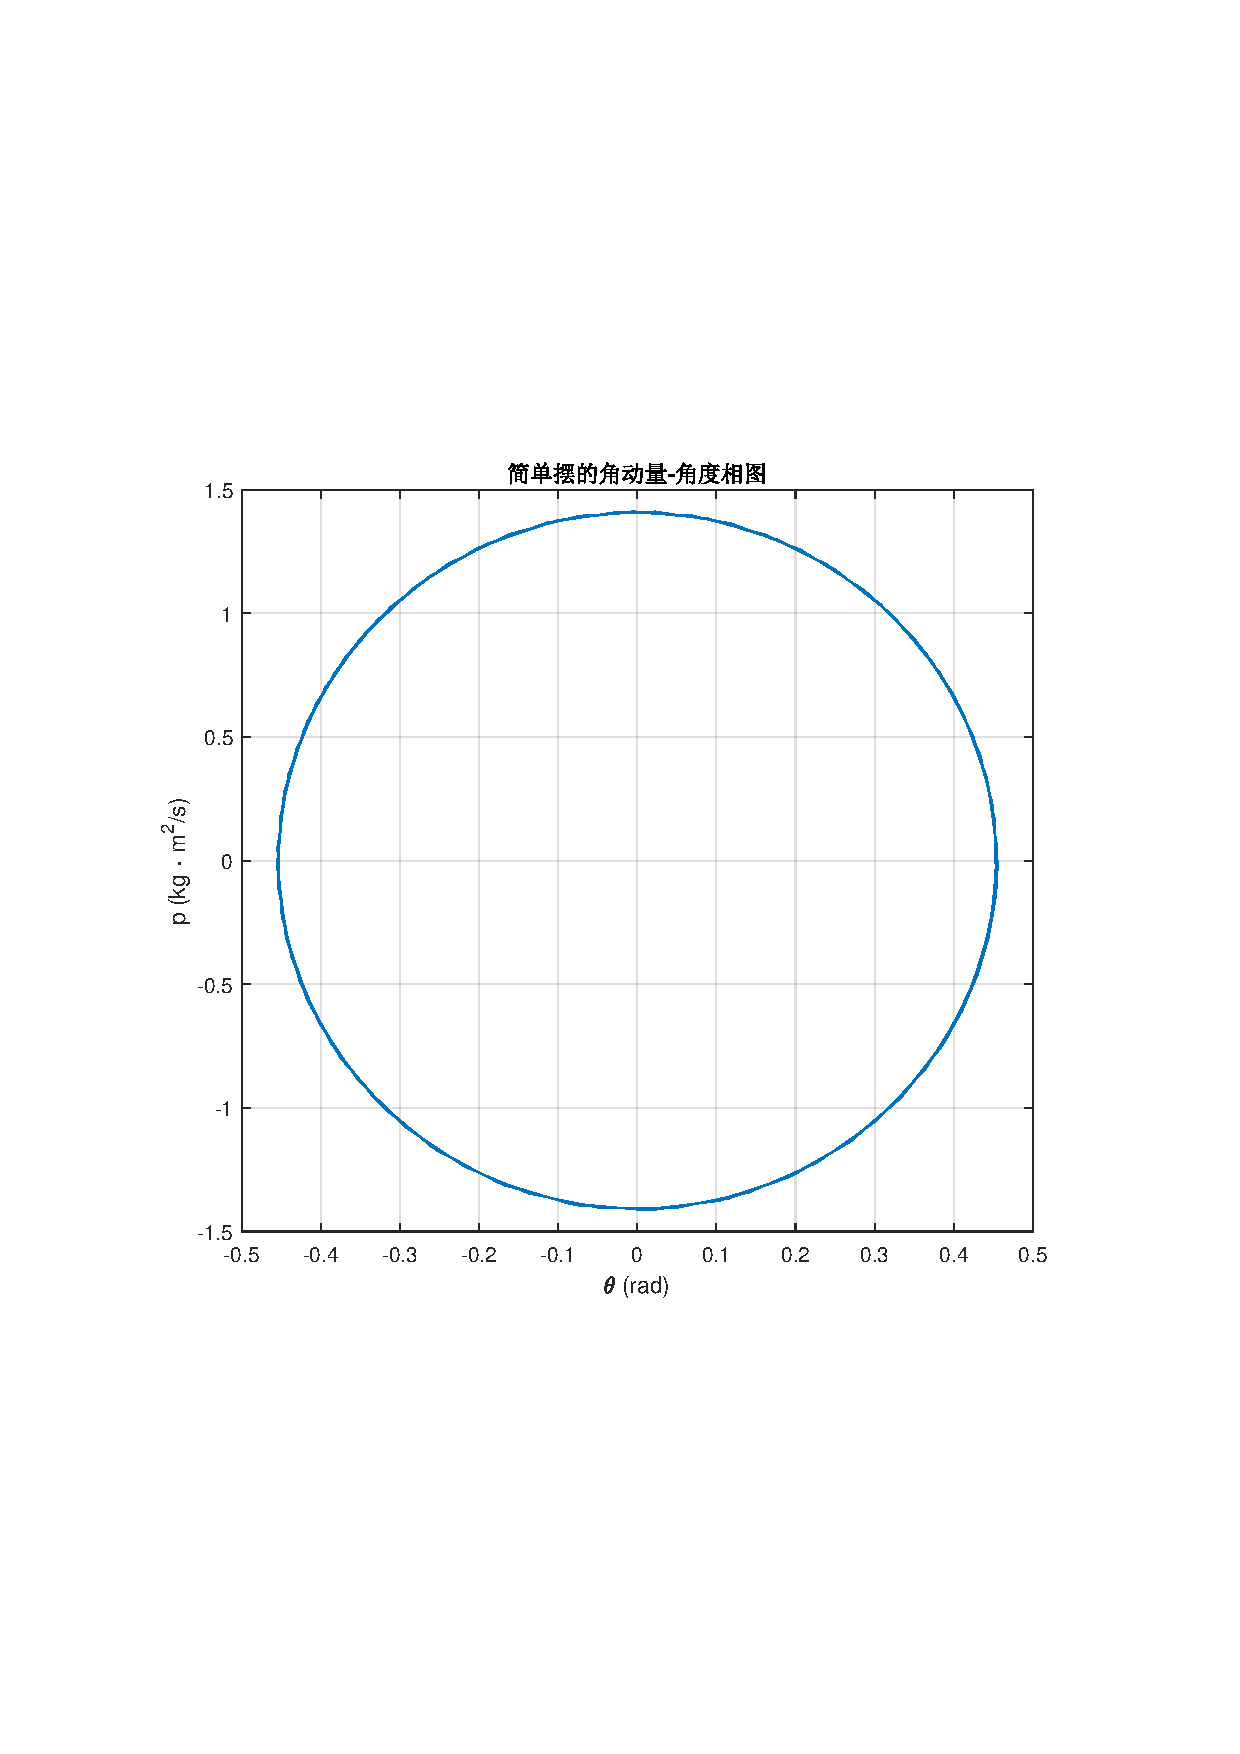
\includegraphics[width=0.5\textwidth,height=0.7\textwidth]{fig/phase-space.pdf}
	\end{figure}
\end{enumerate}

\end{document}